\chapter{Empire, Colonialism and War (1895--1945)}

\section{Japan becomes an empire}

\begin{center}
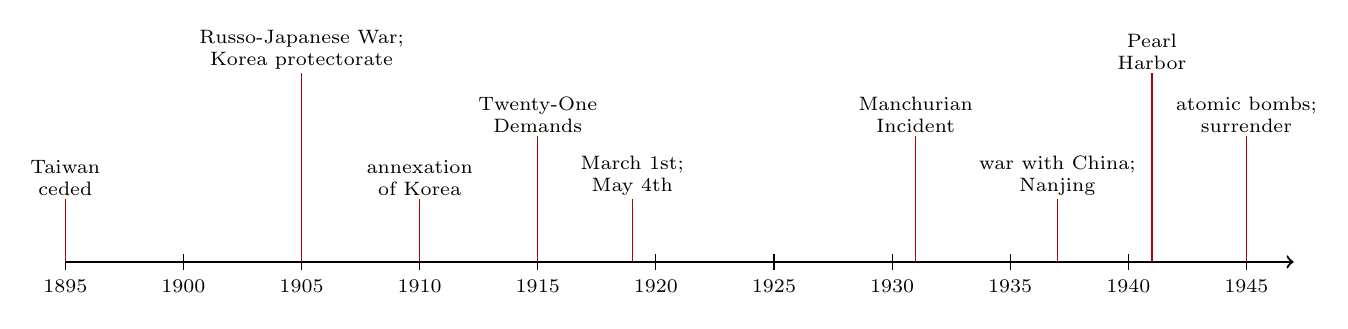
\begin{tikzpicture}[x=0.6cm, y=1cm, every node/.style={font=\scriptsize}]
  \draw[->, thick] (0,0) -- (26,0);
  \foreach \yr in {1895,1900,1905,1910,1915,1920,1925,1930,1935,1940,1945} {
    \pgfmathsetmacro{\x}{(\yr-1895)/2}
    \draw (\x,0.1) -- (\x,-0.1) node[below] {\yr};
  }
  \foreach \yr/\lab/\h in {1895/{Taiwan\\ceded}/0.8, 1905/{Russo-Japanese War;\\Korea protectorate}/2.4,
      1910/{annexation\\of Korea}/0.8, 1915/{Twenty-One\\Demands}/1.6, 1919/{March 1st;\\May 4th}/0.8,
      1931/{Manchurian\\Incident}/1.6, 1937/{war with China;\\Nanjing}/0.8, 1941/{Pearl\\Harbor}/2.4,
      1945/{atomic bombs;\\surrender}/1.6} {
    \pgfmathsetmacro{\x}{(\yr-1895)/2}
    \draw[red!70!black] (\x,0) -- (\x,\h);
    \node[above, align=center, fill=white, inner sep=1pt] at (\x,\h) {\lab};
  }
\end{tikzpicture}
\end{center}

\subsection{Russo-Japanese War (1904--05)}

Rivalry with Russia over Manchuria and Korea led to war. Japan won at Port Arthur and
destroyed the Russian Baltic fleet at Tsushima (1905). The Treaty of Portsmouth
(mediated by Theodore Roosevelt) gave Japan southern Sakhalin, the Liaodong lease and the
South Manchurian Railway, and recognized Japan's ``paramount interest'' in Korea.

\begin{remark}
It was the first modern victory of an Asian power over a European one. It inspired
nationalists from India to Egypt, even as Japan was itself becoming a colonizer of Asians.
This tension (liberator or conqueror?) runs through the whole period.
\end{remark}

\subsection{Taiwan (1895--1945)}

Taiwan was Japan's first colony. After armed resistance was crushed, the colonial
government built railways, ports, sugar industry, public health and schools. Indigenous
peoples resisted (the Musha/Wushe Incident, 1930). Postwar memory of Japanese rule in
Taiwan is relatively mixed or even positive compared with Korea, partly because the
Nationalist (KMT) regime that followed was itself experienced as harsh (the 228 Incident,
1947).

\section{Korea under Japanese rule (1910--1945)}

Korea became a protectorate in 1905 (Itō Hirobumi as Resident-General; he was
assassinated by the Korean nationalist An Jung-geun in Harbin in 1909) and was annexed in
1910. Scholars divide colonial rule into three phases.

\begin{center}
\begin{tabular}{lp{4.2cm}p{7cm}}
\toprule
Phase & Name & Main features \\
\midrule
1910--1919 & ``military rule'' & military police; land survey (much land to Japanese
companies and the Oriental Development Company); Korean newspapers and organizations
banned \\
1919--1931 & ``cultural rule'' & after the March First Movement: some Korean-language
newspapers (\emph{Dong-A Ilbo}, \emph{Chosun Ilbo}), limited associations; continued
surveillance; industry begins \\
1931/37--1945 & assimilation and wartime mobilization & \emph{naisen ittai} (``Japan and
Korea as one body''); Shinto shrine worship compulsory; Korean language banned in schools;
forced name change to Japanese-style names (\ja{創氏改名}, 1940); labour and military
mobilization; ``comfort women'' \\
\bottomrule
\end{tabular}
\end{center}

\subsection{The March First Movement (1919)}

Inspired partly by Woodrow Wilson's language of national self-determination, 33 religious
leaders (Cheondogyo, Christian and Buddhist) signed a Declaration of Independence on 1 March
1919. Peaceful demonstrations spread across the country; perhaps a million people took
part. The Japanese response was brutal (thousands killed, including the young student Yu
Gwan-sun, who died in prison). A Provisional Government was set up in Shanghai.

\begin{important}[The colonial modernity debate]
\begin{itemize}
  \item \textbf{Nationalist view}: colonialism was exploitation and cultural genocide;
        Korean development was stunted.
  \item \textbf{``Colonial modernization'' view} (controversial): railways, industry and
        schools laid foundations for postwar growth.
  \item \textbf{``Colonial modernity''} (a middle view common in North American scholarship):
        modern institutions did arrive, but in a colonial form designed for Japanese
        purposes; Koreans also used them to build their own modern identities. Avoid both
        ``everything was destroyed'' and ``colonialism helped''.
\end{itemize}
\end{important}

\subsection{``Comfort women''}

From the early 1930s to 1945 the Japanese military organized a system of sexual slavery
for its troops. Tens of thousands of women (estimates vary widely, often cited as up to
200\,000), many Korean but also Chinese, Filipino, Indonesian, Dutch and others, were
recruited by deception or force. The issue became public in 1991 when Kim Hak-sun testified.
It remains a central point of dispute between Korea and Japan (the 1993 Kōno Statement, the
2015 agreement, the statues of girls outside the Japanese embassy in Seoul and elsewhere).

\section{China: revolution and fragmentation}

\begin{itemize}
  \item \textbf{1911 Revolution}: the Qing fell; the Republic of China was founded
        (1912) with \textbf{Sun Yat-sen} briefly president, then power passed to the
        general Yuan Shikai.
  \item \textbf{Warlord era} (1916--1928): central authority collapsed.
  \item \textbf{May Fourth Movement} (1919): students protested the Versailles decision to
        give Germany's rights in Shandong to Japan. The wider New Culture Movement attacked
        Confucianism, promoted vernacular writing (\zh{白话}, báihuà; Lu Xun's ``A Madman's
        Diary'', 1918) and ``Mr.\ Science and Mr.\ Democracy''.
  \item The \textbf{Chinese Communist Party} (CCP, 1921) and the \textbf{Nationalist Party}
        (Guomindang/KMT) cooperated, then split violently (Shanghai, 1927). Chiang Kai-shek
        unified much of China under the KMT by 1928.
\end{itemize}

\section{Japan's road to war}

\begin{enumerate}
  \item \textbf{Taishō democracy} (1910s--20s): party cabinets, universal male suffrage
        (1925), but also the Peace Preservation Law (1925) against radicals.
  \item The \textbf{Depression} hit rural Japan hard; many blamed party politicians and
        big business.
  \item \textbf{Manchurian Incident} (1931): Kwantung Army officers staged a bombing of the
        railway near Mukden as a pretext, seized Manchuria without government approval, and
        set up the puppet state of Manchukuo (1932) under the last Qing emperor Puyi. Japan
        left the League of Nations (1933).
  \item Military influence grew through assassinations and attempted coups (1932, 1936).
  \item \textbf{Marco Polo Bridge Incident} (July 1937) began full-scale war with China.
\end{enumerate}

\subsection{The Second Sino-Japanese War (1937--1945)}

\begin{itemize}
  \item \textbf{Nanjing Massacre} (December 1937 -- January 1938): after taking the
        Nationalist capital, Japanese troops killed large numbers of prisoners and civilians
        and committed mass rape. Chinese estimates are around 300\,000 dead; the event and its
        numbers remain politically contested.
  \item The KMT retreated to Chongqing; the CCP built base areas in the north (Yan'an) and
        grew from about 40\,000 to over a million members by 1945.
  \item \textbf{Unit 731}: biological warfare experiments on prisoners in Manchuria.
\end{itemize}

\subsection{The Pacific War}

To secure oil and resources after US embargoes, Japan attacked Pearl Harbor and European
colonies in Southeast Asia (December 1941), proclaiming a \textbf{Greater East Asia
Co-Prosperity Sphere} to liberate Asia from Western imperialism. In practice, occupation
was often harsh. After Midway (1942) the tide turned. The firebombing of Tokyo (March
1945), the battle of Okinawa, the atomic bombings of \textbf{Hiroshima} (6 August) and
\textbf{Nagasaki} (9 August), and the Soviet invasion of Manchuria led to Japan's surrender,
announced by the emperor on 15 August 1945.

\begin{aside}
August 15 is remembered very differently: in Korea it is Liberation Day
(\ko{광복절}, Gwangbokjeol, ``restoration of light''); in Japan it is ``the day the war
ended'' (\ja{終戦の日}, shūsen no hi); China marks victory on September 3. Even the word
for the event reveals the perspective.
\end{aside}

\section{War memory}

\begin{center}
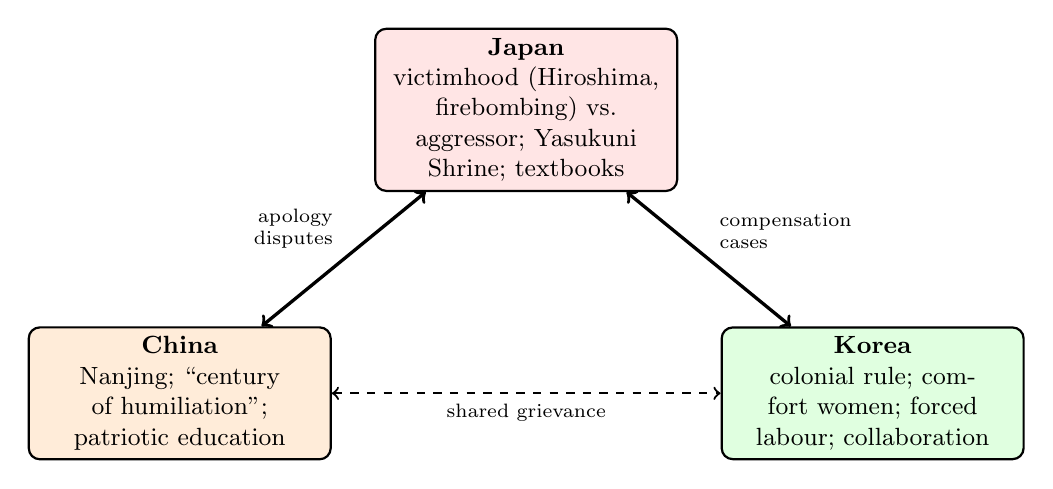
\begin{tikzpicture}[b/.style={draw, thick, rounded corners, text width=3.6cm, align=center, font=\small}]
  \node[b, fill=red!10] (j) at (0,2.4) {\textbf{Japan}\\victimhood (Hiroshima, firebombing) vs.\ aggressor; Yasukuni Shrine; textbooks};
  \node[b, fill=orange!15] (c) at (-4.4,-1.2) {\textbf{China}\\Nanjing; ``century of humiliation''; patriotic education};
  \node[b, fill=green!12] (k) at (4.4,-1.2) {\textbf{Korea}\\colonial rule; comfort women; forced labour; collaboration};
  \draw[<->, very thick] (j) -- node[above left, font=\scriptsize, align=right] {apology\\disputes} (c);
  \draw[<->, very thick] (j) -- node[above right, font=\scriptsize, align=left] {compensation\\cases} (k);
  \draw[<->, thick, dashed] (c) -- node[below, font=\scriptsize] {shared grievance} (k);
\end{tikzpicture}
\end{center}

\begin{itemize}
  \item \textbf{Yasukuni Shrine} in Tokyo enshrines Japan's war dead, including 14 Class-A war
        criminals (added secretly in 1978). Prime-ministerial visits provoke protests from
        China and Korea.
  \item \textbf{Textbooks}: controversies since the 1980s over how Japanese school textbooks
        describe the invasion of China and colonial rule.
  \item \textbf{Apologies}: the Murayama Statement (1995) expressed ``deep remorse'' and a
        ``heartfelt apology''; critics in Asia point to contradictory statements by other
        politicians.
\end{itemize}

\section*{Summary}
\begin{itemize}
  \item Japan acquired Taiwan (1895), Korea (1905/1910) and Manchuria (1931--32).
  \item Korean colonial rule: military rule, ``cultural rule'' after March First (1919),
        then assimilation and wartime mobilization.
  \item China: 1911 revolution, warlords, May Fourth, KMT--CCP rivalry, war with Japan from
        1937.
  \item The Pacific War ended with the atomic bombings and surrender on 15 August 1945.
  \item War memory (Nanjing, comfort women, Yasukuni, textbooks) remains politically
        explosive.
\end{itemize}
